\chapter{Características de las herramientas analizadas} 

\label{carac_herramientas_anali}

Las características analizadas en cada una de las herramientas son las siguientes:

\begin{itemize}
\item Información general
\item Uso. Explicación sobre el funcionamiento de la herramienta
\item Extensibilidad. Capacidad de conexión con otras herramientas
\item Integración. Capacidad para desplegar el chatbot
\item Ejemplos
\end{itemize}


\section{AIML}

\subsection*{Información general}

El lenguaje de programación AIML (Artificial Intelligence Markup Language) fue desarrollado por el doctor Richard Wallace y la comunidad de código abierto Alicebot en la segunda mitad de los años 90. AIML es un lenguaje basado en etiquetas, al igual que los lenguajes HTML y XML. En concreto, el lenguaje AIML se basó en gran medida en el lenguaje XML. Este parecido entre lenguajes no es una casualidad, si nos fijamos en el entorno de la época en la que se desarrolló AIML, a finales de la década de 1990 se produjo la explosión de la \gls{world_wide_web}. Esta explosión trajo consigo al lenguaje HTML, que surgió como un lenguaje simple que sirviese como estándar para la creación de páginas web. El objetivo de HTML era que cualquier persona con pocos conocimientos informáticos fuese capaz de crear una página web. Esta filosofía de estándar de una tecnología y de simpleza la tomaron como ejemplo los creadores de AIML durante su desarrollo, intentando que AIML se convirtiese en un estándar en la creación de chatbots y que además fuese accesible al mayor número de usuarios. Además del lenguaje HTML, durante la década de 1990 se creó el lenguaje XML, que también se convirtió en un estándar.

Actualmente, al igual que le ha pasado al lenguaje HTML, el lenguaje AIML se ha ido actualizando con el tiempo, añadiéndole nuevas funcionalidades que permitiesen producir chatbots más complejos, acorde al incremento de requisitos en los chatbots que ha ido surgiendo con el paso de los años. En el momento de la realización de este TFG, la última versión publicada de AIML es la versión 2.1\ . Al producir agentes conversacionales con AIML, estos agentes no se convierten en cajas negras, por lo tanto, son más transparentes al programador que los generados con otras plataformas más grandes, ya que con AIML se crean chatbots basados en reglas. AIML se puede escribir en casi cualquier lenguaje natural.

\subsection*{Uso}

Para generar un chatbot con AIML es necesario generar una serie de archivos, que contendrán el estado y la configuración del bot.

En el estado del chatbot podemos distinguir el estado del bot y el estado del cliente. El estado del bot se define usando valores globales para las propiedades del bot, cada bot tendrá sus propiedades. El estado del cliente se define empleando variables locales, cada cliente tendrá su estado específico.

La configuración del bot se define en los archivos AIML, en los archivos Learnf, en los Sets y en los Maps. Dentro de los archivos AIML se define la lógica del chatbot a base de añadir reglas, además en estos archivos se pueden realizar conexiones con otros chatbots definidos por otra serie de archivos. Dentro de los archivos Learnf se guardan las categorías aprendidas por el chatbot cuando en un template AIML se activa una etiqueta. Las categorías aprendidas son globales a todos los clientes del chatbot. Dentro de los archivos Set se define un conjunto de cadenas. Dentro de los archivos Map se define un mapeo de cadena a cadena.

Según el estándar de AIML, esta serie de archivos se pueden definir dónde y cómo quiera el creador del chatbot.

Dado que AIML es solamente un lenguaje de programación, es necesario un \gls{framework} para la creación del agente conversacional, como pueden ser algunos intérpretes y bibliotecas de código abierto (Python, Node JS, Java) o servicios web (Pandorabots).

Si se elige la opción de usar intérpretes y bibliotecas de código abierto, disponemos de las siguientes posibilidades:

\begin{itemize}
\item Python $\rightarrow$ Program-Y \footnote{\url{https://github.com/keiffster/program-y}}
\item Node JS $\rightarrow$ aimlinterpreter
\footnote{\url{https://www.npmjs.com/package/aimlinterpreter}}
\item Java $\rightarrow$ Program AB \footnote{\url{https://code.google.com/archive/p/program-ab}}
\end{itemize}

Si se elige la opción de usar servicios web como Pandorabots, uno de los más populares actualmente, se podrá alojar el chatbot en la plataforma y se podrá hacer uso de todas sus funcionalidades. Si nos centramos en Pandorabots disponemos de un editor de AIML, un editor de interfaces, control de versiones a través de Github, chatlogs, conversor de texto a voz y viceversa, posibilidad de añadir un personaje 3D como interacción con el chatbot, integración con RESTful \glspl{API} y muchos más, según se indica en su página oficial \cite{RefWorks:RefID:14-pandorabots:}.

Muchas de estas funcionalidades depende del tipo de cuenta que se disponga en Pandorabots.

\newpage

\begin{figure}[h]
\centering
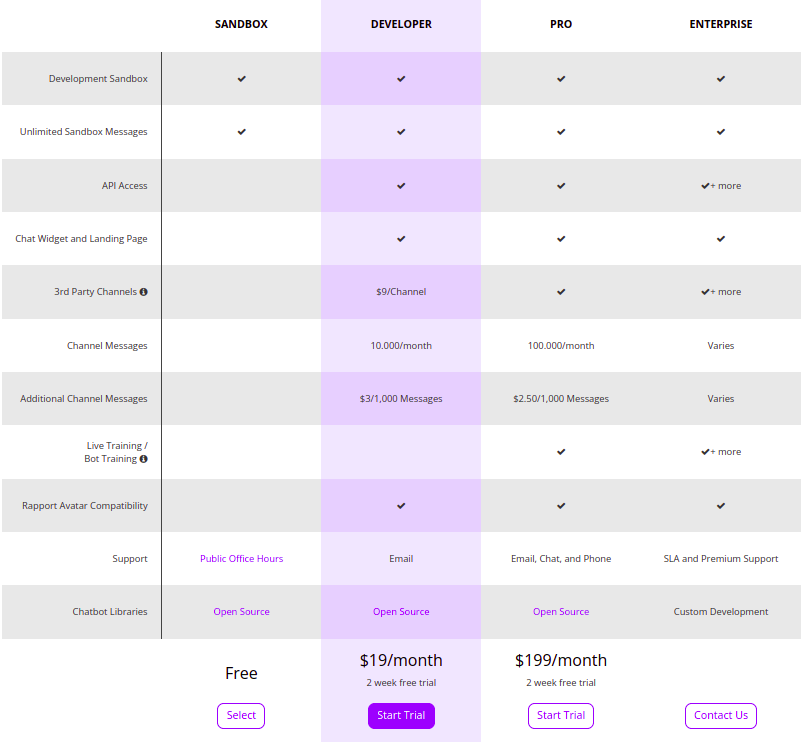
\includegraphics[width=1.0\textwidth]{imagenes/02_EstadoDelArte/cuentas_pandorabots.png}
\begin{center}
Fuente: \url{https://developer.pandorabots.com/home.html}
\end{center}
\caption{Cuentas disponibles en Pandorabots}
\label{fig:cuenta_pandorabots}
\end{figure}

En la Figura \ref{fig:cuenta_pandorabots} podemos comprobar como con la cuenta gratuita no disponemos de todas las funcionalidades anteriormente descritas.

\subsection*{Extensibilidad}

Dado que hay muchos \glspl{framework} para la creación de un chatbot con AIML, dependerá del \gls{framework} elegido la cantidad de posibilidades de conexiones con \glspl{API} o servicios externos al chatbot.

Para que AIML sea flexible y extensible dispone de la posibilidad de integrar sus propias \glspl{API}, bases de datos o también se pueden crear etiquetas propias; pero para ello se debe tener cierto nivel con el lenguaje de programación AIML.

Si optamos por servicios web como Pandorabots para poder disponer de conexión con servicios externos al servicio web o con \glspl{API} se debe disponer de una cuenta de pago, no basta con la versión gratuita de Pandorabots.

\subsection*{Integración}

Si optamos por servicios web como Pandorabots, al igual que pasa con la extensibilidad, será necesaria una cuenta de pago para poder integrar nuestro chatbot en plataformas de mensajería como Facebook Messenger, Twitter, Telegram y muchos más.

Pero si optamos por \glspl{framework} de código abierto, hay una multitud de posibilidades, tantas como el nivel de conocimientos que tenga el creador del chatbot. Un ejemplo puede ser con Node JS, donde podríamos desplegar el chatbot en cualquier página web a través de una interfaz web que enviase peticiones al servidor creado con Node JS que aloja al chatbot.

\subsection*{Ejemplos}

Algunos ejemplos de chatbot implementados con AIML son los siguientes:

\begin{itemize}
\item \textbf{Rosie}. Chatbot base basado en ALICE 2.0 \footnote{\url{https://github.com/pandorabots/rosie}}
\item \textbf{Cathy}. Chatbot para Discord basado en Python 3 y AIML \footnote{\url{https://github.com/DevDungeon/Cathy}}
\end{itemize}


\section{IBM Watson}

\subsection*{Información general}

IBM Watson es un \gls{portfolio} de IBM de aplicaciones, herramientas y soluciones preparadas para la empresa, diseñado para reducir los costes y los obstáculos de \gls{IA}, además de optimizar los resultados y el uso responsable de la \gls{IA} según se indica en su página oficial \cite{RefWorks:RefID:15-2021ibm}. Aunque en un inicio IBM Watson no era lo que es actualmente y tampoco se buscaba llegar a este punto. Originalmente, IBM Watson surgió como el siguiente gran desafío de la empresa IBM, tras haber salido victorioso de otros grandes desafíos como la victoria de Deep Blue contra Garry Kasparov y el desafío de la supercomputadora Blue Gene. El objetivo que perseguía en sus orígenes Watson era conseguir ganar a competidores humanos en el concurso Jeopardy. Este concurso de televisión estadounidense consistía en un concurso de preguntas sobre una multitud de temas, y los concursantes deberán resolver las preguntas de cada prueba realizando preguntas sobre las pistas que va dando el presentador. Las reglas del concurso obligan a que Watson no únicamente sepa conocimientos sobre los temas que se utilizan en el concurso, sino también a saber efectuar preguntas al presentador basándose en sus pistas, y además saber distinguir cuando la pista del presentador no es cierta. Todos estos requisitos convierten el ganar este concurso en un gran desafío, la empresa IBM se embarcó en este proyecto a mediados de la década del 2000. Finalmente, en el año 2011 se llegó a un acuerdo para la realización del programa, donde compitieron dos grandes ex-concursantes del programa como son Ken Jennings y Brad Rutter contra Watson. Tal y como se indica en el artículo \cite{RefWorks:RefID:16-best2013ibm}, Watson ganó el juego con \$77.147, dejando a Rutter y Jennings con \$21.600 y \$24.000 respectivamente.

Tras la victoria de IBM Watson, se empezó a enfocar y rediseñar a Watson hacia distintos sectores como la medicina, la banca o los agentes conversacionales, entre otras. Los agentes conversacionales es el sector que nos interesa investigar.

Dado que IBM Watson está orientado al mundo empresarial, destaca por su confianza, es decir, Watson es transparente en cuanto a las decisiones basadas en \gls{IA}; también protege la privacidad de los datos y su seguridad. Todas estas características son muy valoradas en cualquier producto empresarial, incluso algunas son imprescindibles.

Otra característica de Watson es su procesamiento del lenguaje natural. Al igual que AIML es multilenguaje, pero Watson lo lleva a un aspecto más complejo, añadiendo la capacidad de analizar datos complejos y no estructurados, como pueden ser códigos de programación o incluso formas de expresión específicas de una modalidad de trabajo. Este procesamiento del lenguaje natural no es algo alcanzable por cualquier empresa. La \gls{IA} de Watson sabe desenvolverse en las situaciones más complejas, como pueden ser situaciones en las que no pueda responder, reenviando la solicitud a un agente humano o hacia algún documento de ayuda; evitando realizar preguntas redundantes facilitando la comunicación y haciéndola más natural; y por último sabe manejar solicitudes ambiguas que son comunes en la comunicación como pueden ser errores ortográficos, cambios de tema, y muchas más situaciones que pueden ser inesperadas para el chatbot en una conversación. Además, IBM Watson intenta mejorar su rendimiento aportando al creador del chatbot información sobre que nuevos temas añadir para mejorar la respuesta a las solicitudes.

Y por último, destaca que Watson trabaja con cualquier servicio en la nube, lo que facilita su integración en las empresas, ya que no será un impedimento el lugar donde residan los datos de la empresa. Y además el trabajar en \gls{cloud} facilitará el trabajo con los datos.

En concreto, en la página oficial de IBM Watson Assistant \cite{RefWorks:RefID:17-ibm} se destaca la rentabilidad del producto, de hasta un 337\% según el Informe TEI de Forrester \cite{RefWorks:RefID:8-iles2020el}; su precisión, de hasta un 14,7\% superior que las soluciones de la competencia según un reciente estudio publicado sobre machine learning \cite{RefWorks:RefID:18-2020watson}; y su fiabilidad, ya que Watson tiene más de 1000 despliegues de clientes en todos los sectores.

\subsection*{Uso}

IBM Watson está pensado para ser utilizado por cualquier persona, da igual que no tenga conocimientos en programación. La creación del chatbot se basa en un editor de arrastrar y soltar. Este editor evita la complejidad de la programación de un chatbot y los posibles errores derivados de esa necesidad de escribir el código en su creación o en alguna modificación que necesite el chatbot. Es posible crear un chatbot sin escribir una sola línea de código.

\begin{figure}[h]
\centering
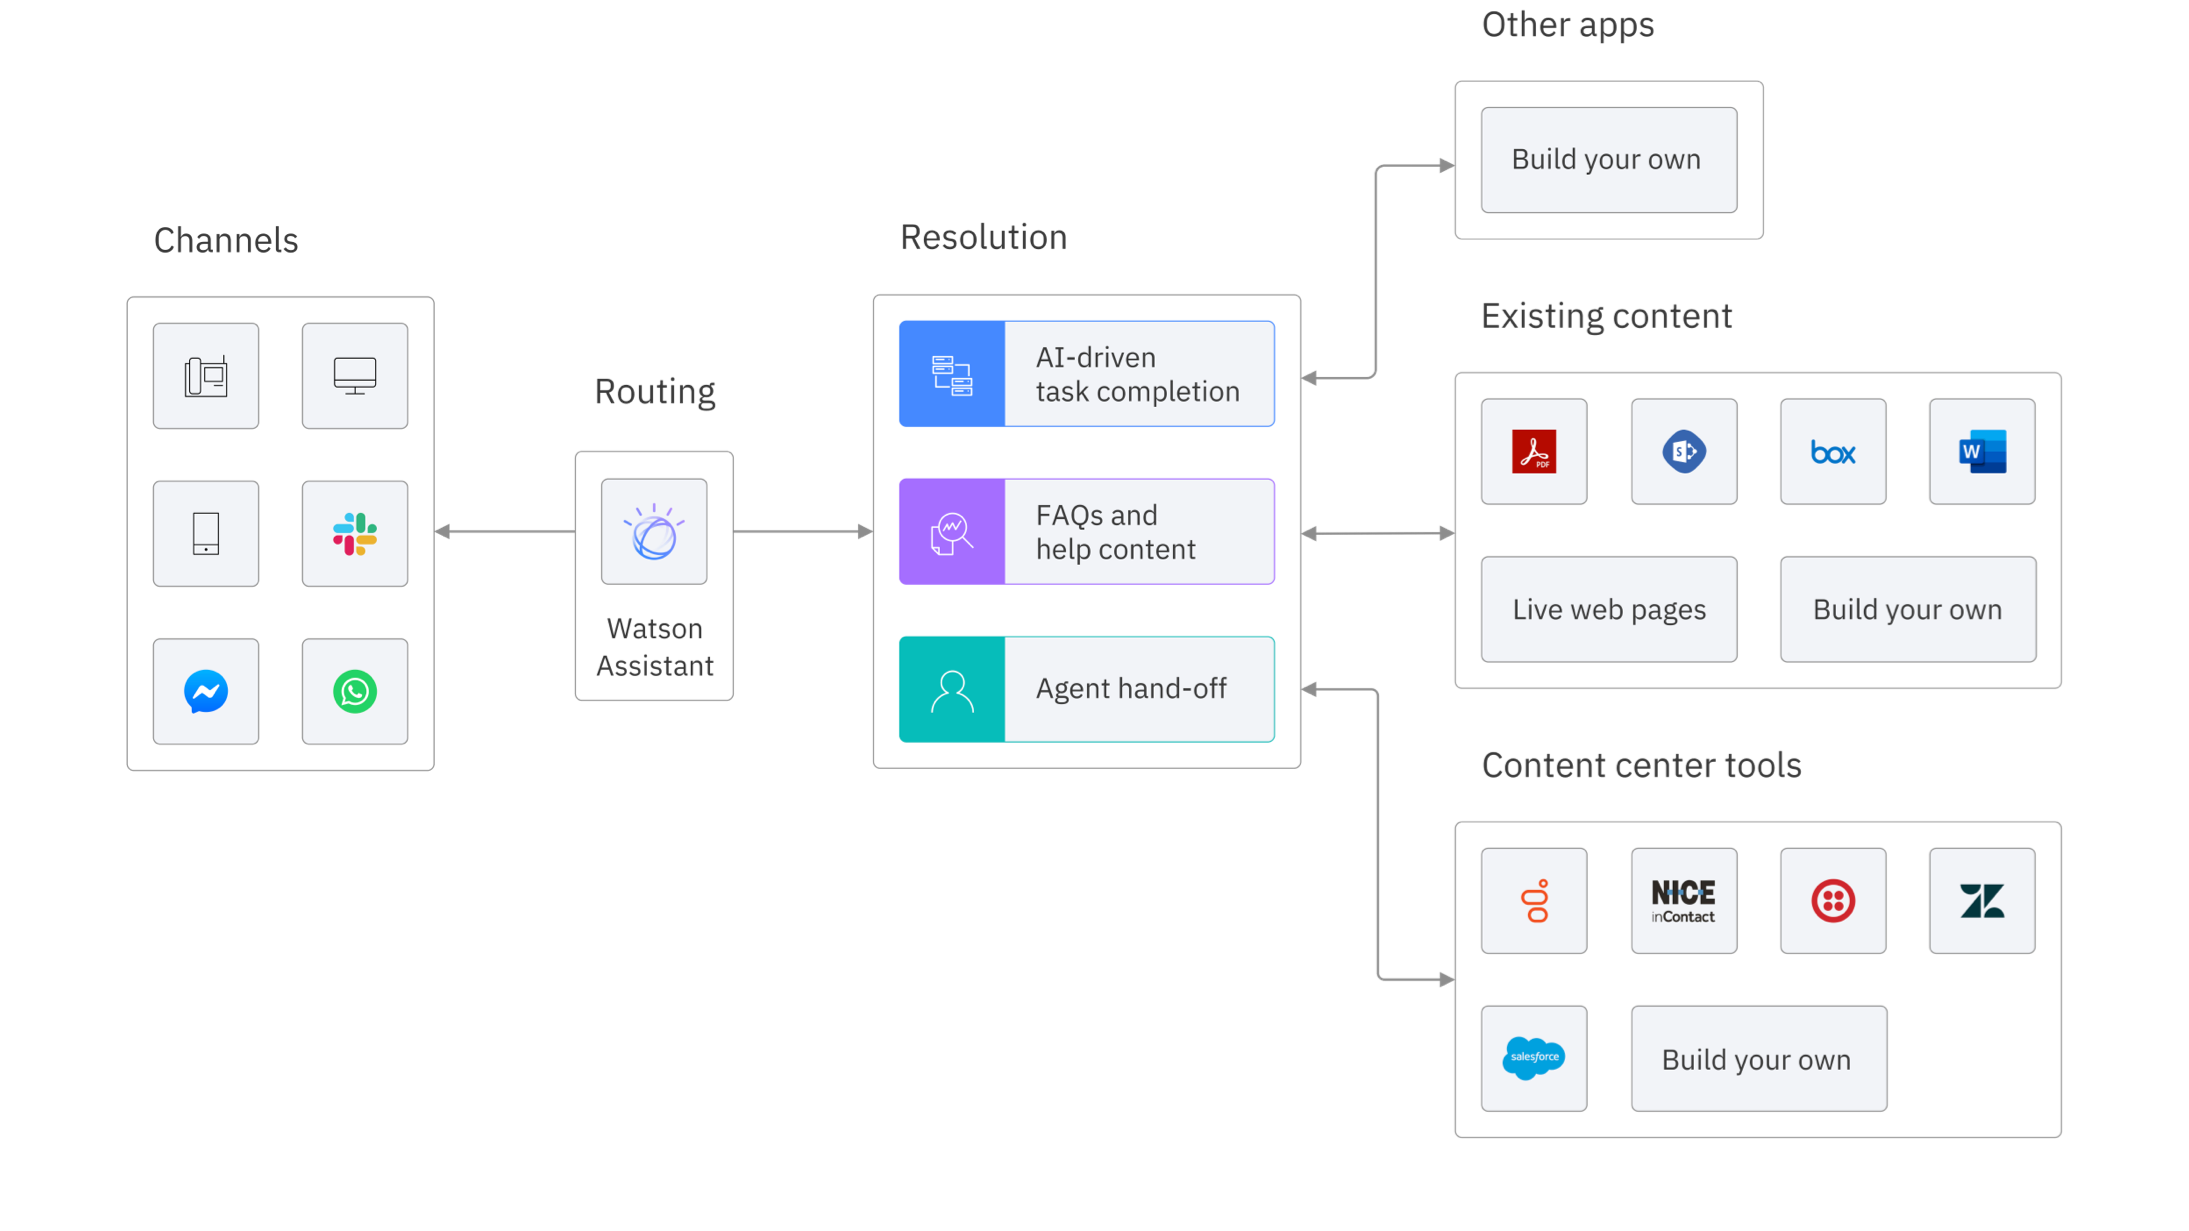
\includegraphics[width=1.0\textwidth]{imagenes/02_EstadoDelArte/editor_IBM_Watson.png}
\begin{center}
Fuente: \url{https://www.ibm.com/es-es/products/watson-assistant}
\end{center}
\caption{Editor de IBM Watson}
\end{figure}

La IA del chatbot es capaz de comprender un tema en cualquier lenguaje natural con unas pocas frases, facilitando la adaptación del chatbot a la funcionalidad que se le quiera dar, adaptándose de forma rápida y precisa al dominio del proyecto.

\subsection*{Extensibilidad}

Como se ha indicado en apartados anteriores, IBM Watson es un \gls{portfolio} de IBM de aplicaciones. En su página oficial \cite{RefWorks:RefID:19-2021productos} se indican las siguientes aplicaciones con las que se puede integrar el chatbot:

\begin{itemize}
\item IBM Watson Discovery
\item IBM Watson Natural Language Understanding
\item IBM Watson Speech to Text
\item IBM Watson Text to Speech
\item IBM Watson Knowledge Studio
\item IBM Watson Language Translator
\item IBM Watson Natural Language Classifier
\end{itemize}

Entre estas aplicaciones se encuentran algunas muy útiles como IBM Watson Discovery para la extracción y búsqueda de información, IBM Watson Speech to Text para transformar la voz a texto escrito gracias a una potente tecnología de machine learning, IBM Watson Language Translator para traducir dinámicamente información, o IBM Watson Knowledge Studio para enseñar a Watson el idioma del dominio del chatbot.

\subsection*{Integración}

El chatbot se puede integrar como un chat web, como contestador de llamadas de teléfono o como un chatbot en una aplicación de mensajería como WhatsApp, Facebook Messenger, SMS y muchos más. Todas estas maneras de integrar el chatbot son muy fáciles de realizar.

\subsection*{Ejemplos}

Algunos ejemplos de chatbot implementados con Watson son los siguientes:

\begin{itemize}
\item \textbf{Nanci. Chatbot desarrollado por la empresa GM Financial} \footnote{\url{https://www.gmfinancial.com/en-us/company/newsroom/chatbot.html}}
\item \textbf{Chatbot desarrollado por la empresa Bradesco} \footnote{\url{https://www.ibm.com/watson/stories/bradesco}}
\item \textbf{CARL. Chatbot desarrollado por la empresa Siemens} \footnote{\url{https://www.ibm.com/es-es/products/watson-assistant/client-stories}}
\item \textbf{Chatbot desarrollado por la empresa Humana} \footnote{\url{https://www.ibm.com/watson/stories/humana}}
\end{itemize}


\section{Google Dialogflow}\label{subsec:dialogflow}

\subsection*{Información general}

Dialogflow pertenece a la empresa Google, aunque no fue desarrollada originalmente por ella. Google adquirió API.AI en el año 2016 y le cambió el nombre a Dialogflow. Desde su adquisición, Google ha mejorado Dialogflow gracias a sus técnicas de \gls{IA} de gran calidad. Esta plataforma es una de las más utilizadas para la creación de chatbots junto con IBM Watson, aunque a diferencia de Watson, Dialogflow está enfocado tanto para el mundo empresarial como para usuarios particulares que están empezando en el mundo de los chatbots. Esta variedad en la complejidad del chatbot es posible gracias a una interfaz que permite crear un chatbot con unos mínimos conocimientos técnicos, únicamente será necesario introducir las frases de las preguntas y de las respuestas para construir el chatbot. Y si se quiere generar un chatbot más complejo, podemos introducirnos en la configuración del chatbot o integrar más funcionalidades que aumenten su complejidad.

Dentro de Dialogflow existen dos tipos de agentes, los Agentes de ES y los agentes de CX. Dentro de los agentes de ES existen dos ediciones, la edición de prueba y la edición Essentials. Con la versión de prueba no se puede acceder a los servicios de Google Cloud, pero las entradas y salidas son gratuitas; mientras que con la versión Essentials si se puede acceder a esos servicios, pero las entradas y salidas del agente empezarán a costar dinero. Entre la versión Essentials y la versión CX la principal diferencia es que en la versión CX la relación entre los intents se define mediante un diagrama de flujo, mientras que en la versión Essential la relación entre los intents se define mediante los contextos. La limitación de los contextos es que no posibilitan la relación de varios intents con otro intent. La versión CX ha sido lanzada hace unos pocos meses, por lo que es algo novedosa y es útil para aquellos que quieran realizar un chatbot algo más complejo o que ya tengan experiencia con la plataforma. La versión Essentials está más enfocada a agentes de complejidad media y la versión CX está más enfocada a agentes de complejidad alta. Aunque la curva de aprendizaje es más suave en la edición CX, la edición CX no dispone actualmente de todas las funcionalidades presentes en la edición Essentials.

\subsection*{Uso}

Para empezar a crear un chatbot con Dialogflow será necesaria una cuenta Google. Los apartados claves para la creación de un bot son Intents y Entities.

Dentro del apartado Intents se generan los distintos intents a usar en el chatbot, cada intent es un estado al que accede el chatbot si se cumple el contexto y se detecta una de las frases de entrenamiento del intent. Los contextos sirven para guardar información adquirida que puede resultar útil durante la conversación, como el nombre del usuario que está utilizando el chatbot; además de la información que se quiere conservar, también se puede indicar durante cuento tiempo se estima que es útil esa información, también llamado lifespan. Dentro de cada intent se debe también definir las posibles respuestas que envía el chatbot si se activa el intent. Y por último a cada intent se le pueden añadir eventos. Por defecto, en el apartado Intents vienen creados los siguientes intents:

\begin{itemize}
\item Default Fallback Intent: Intent para cuándo el chatbot no reconoce la pregunta
\item Default Welcome Intent: Intent para dar la bienvenida al chatbot
\end{itemize}

Dentro del apartado Entities se generan las distintas entidades. Una entidad es un conjunto de ejemplos sobre un tema, por ejemplo, la entidad países contiene los siguientes elementos: España, Francia, Italia, etc. Cuando se define una entidad se deben indicar los elementos que la forman, pero adicionalmente se puede indicar los sinónimos de los elementos, este añadido le dará una mayor naturalidad a la conversación al hacer que los textos no sean tan estáticos.

Otro apartado importante para el desarrollo del chatbot es el apartado Training, donde se podrán analizar las conversaciones que se han realizado con el chatbot e indicar si se ha respondido adecuadamente o no, esta acción de aceptación o no hará que el chatbot sea más preciso con sus respuestas. Si se acepta una respuesta, si la pregunta hecha por el usuario no se encuentra entre las preguntas del intent activado, se añade a la lista de preguntas del intent.

\subsection*{Extensibilidad}

Dialogflow permite integrar un \gls{webhook}. Este \gls{webhook} puede estar alojado tanto en un servidor externo como en Google Cloud. Si se opta por la opción de Google Cloud, para lo que es necesario una cuenta Google de pago, se pueden añadir los archivos que componen el \gls{webhook} en el apartado Fulfillment dentro de un editor en línea. Si se opta por la opción de un servidor externo, tanto si es local como si es en una plataforma en la nube, se deberá añadir la URL del servidor web en el mismo apartado que se indicó anteriormente. La conexión con el servidor externo se realizará mediante el envío de peticiones tipo POST. Estas peticiones contendrán la información en formato JSON. Para que la información se envíe al servidor, independientemente de la opción que se elija, se debe activar en los intents elegidos la opción del \gls{webhook}, de esta forma cuando se active el intent se enviará una petición al servidor web.

Una vez se tenga una conexión con un servidor web, dentro de este servidor se podrán añadir más funcionalidad, como BBDD o interpretes de AIML, que permitirán seguir extendiendo el chatbot.

\subsection*{Integración}

El chatbot se puede integrar en canales de telefonía, como Twilio; en canales de mensajería, como Telegram, Facebook Messenger o Twitter; en canales de videollamadas, como Skype; y en páginas web a modo de chat web.

\subsection*{Ejemplos}

Algunos ejemplos de chatbot implementados con Dialogflow son los siguientes:

\begin{itemize}
\item \textbf{SAM. Chatbot desarrollado por la empresa Ubisoft} \footnote{\url{https://www.hd-tecnologia.com/ubisoft-ia-personal-sam-primer-asistente-gaming}}
\item \textbf{Chatbot desarrollado por la empresa Dominos Pizza} \footnote{Caso de estudio de Dominos Pizza \cite{RefWorks:RefID:10-domino's-case-study}}
\item \textbf{Chatbot desarrollado por la empresa Malaysia Airlines} \footnote{\url{https://cloud.google.com/customers/malaysia-airlines}}
\end{itemize}


\section{Rasa Stack}

\subsection*{Información general}

Rasa Stack es un conjunto de herramientas de aprendizaje automático de código abierto para el desarrollo de chatbots. Rasa Stack está desarrollado por una comunidad de personas pertenecientes a muchos lugares del mundo, de modo que esta plataforma, a diferencia de las dos anteriores, no está respaldada por ninguna de las grandes empresas tecnológicas como pueden ser Google o IBM. Pero esto no quiere decir que no sea una buena plataforma, ya que ha sido probada por grandes empresas como AIRBUS, TOYOTA o Adobe.

En su página oficial \cite{RefWorks:RefID:20-2020rasa} se destaca la gran personalización que pueden alcanzar los chatbots en esta plataforma.

Dentro de Rasa Stack se pueden distinguir dos tipos de cuenta, la cuenta para empresas (Rasa Enterprise) y la cuenta gratuita (Rasa Open Source o Rasa X). La diferencia entre Rasa Open Source y Rasa X es que Rasa X no es de código abierto, mientras que Rasa Open Source, como indica su nombre, si es de código abierto. La cuenta para empresas proporciona funcionalidades muy útiles para productos empresariales como pueden ser realizar análisis del chatbot, acceso con roles a la plataforma, disponibilidad de un soporte de calidad, y mucho más.

En Rasa Stack se destaca que los chatbots creados en esta plataforma no se convierten en \glspl{caja_negra}, sino que el funcionamiento del chatbot es transparente, por lo tanto, se tiene total acceso a la configuración de todo el chatbot, incluido el modelo usado en el entrenamiento del bot.

\subsection*{Uso}

Al igual que pasa en Dialogflow, Rasa Stack mantiene un contexto de la conversación, donde se guarda información proporcionada por el usuario, lo que permite una conversación más natural al no hacer preguntas redundantes.

La creación del chatbot se divide en dos módulos, Rasa NLU y Rasa Core. La plataforma proporciona unas \gls{NLU}, estas \gls{NLU} se pueden entrenar sobre la base de una lista de mensajes, a cada mensaje se le asignará una intención y las entidades que contiene. Una vez está entrenado el módulo \gls{NLU}, se procede a configurar el módulo Rasa Core, que es el encargado de confeccionar la respuesta del chatbot a la pregunta identificada por el módulo Rasa NLU. La configuración de Rasa Core consiste en escribir las respuestas de los distintos intents, definir el dominio del chatbot, definir la conexiones con \glspl{API}, y definir el modelo de gestión del diálogo, por ejemplo, una \gls{CNN}, citando además las políticas que se van a usar.

\subsection*{Extensibilidad}

La transparencia que tienen los chatbots permiten conectar con él muchas \glspl{API} externas que suman más funcionalidades aparte de las que ya proporciona la plataforma. Y al igual que pasa con Dialogflow, se puede conectar a un servidor web y a este servidor conectar las \glspl{API}.

\subsection*{Integración}

Tal y como se indica en su página oficial \cite{RefWorks:RefID:20-2020rasa}, un chatbot creado con Rasa Stack se puede integrar en canales como IVR, chat y SMS. Además, se indica que Rasa Stack admite 10 canales de mensajería integrados, como pueden ser Telegram, Facebook Messenger, Slack y algunos más; y que adicionalmente proporciona un punto de conexión con cualquier plataforma de comunicación, como puede ser un servidor web.

\subsection*{Ejemplos}

Algunos ejemplos de chatbot implementados con Rasa Stack son los siguientes:

\begin{itemize}
\item \textbf{Djingo. Chatbot desarrollado por la empresa Orange} \footnote{\url{https://rasa.com/customers/orange}}
\item \textbf{Chatbot desarrollado por la empresa TMobile} \footnote{\url{https://rasa.com/customers/t-mobile}}
\item \textbf{Chatbot desarrollado por la empresa Helvetia} \footnote{\url{https://rasa.com/customers/helvetia}}
\end{itemize}


\section{GPT-3}

\subsection*{Información general}

GPT-3 (Generative Pre-trained Transformer 3) es un conjunto de modelos de \gls{IA} desarrollados por la empresa OpenAI en el año 2020. Este modelo es la tercera generación de estos modelos de inteligencia artificial. En concreto, este último modelo tiene 175 billones de parámetros, lo cual es una potencia impresionante que le permite generar texto que parece escrito por humanos y no por máquinas, es incluso capaz de escribir código. GPT-3 se ha visto potenciado por la inversión de Microsoft entre otros. Este modelo ha revolucionado el procesamiento y la generación de lenguaje natural. Esta última generación es de pago, cobrando cada cierta cantidad de tokens analizados, en concreto cada 1000 tokens actualmente, según se indica en su página de precios \cite{RefWorks:RefID:21-openai.}. Un token es un conjunto de palabras o un conjunto de letras, su tamaño depende también del lenguaje que se esté usando. Si se quiere saber más sobre los tokens se puede emplear la herramienta Tokenizer \footnote{\url{https://beta.openai.com/tokenizer}}, que nos proporciona OpenAI, para calcular el número de tokens en una frase. Algo importante es que únicamente se paga por lo que se emplea, no como en otras páginas que independientemente de lo que se emplee un servicio se paga una cuota fija.

Como se ha indicado anteriormente, GPT-3 es un conjunto de modelos. Según se indica en su página web \cite{RefWorks:RefID:22-modelos} existen los siguientes modelos:

\begin{itemize}
\item Davinci
\item Curie
\item Babbage
\item Ada
\end{itemize}

La diferencia entre los distintos modelos son su potencia, velocidad y coste por token. El modelo Davinci es el más potente y el más caro, mientras que el modelo Ada es el más rápido y barato.

Las posibles aplicaciones de GPT-3, según su página de ejemplos \cite{RefWorks:RefID:23-openai.}, son las siguientes:

\begin{itemize}
\item Generación de lenguaje natural
\item Clasificación
\item Generación de código
\item Chatbot
\item Traducción (tanto código como lenguaje natural)
\end{itemize}

La aplicación de GPT-3 como un chatbot se explicará más en detalle en el siguiente apartado.

Un problema de GPT-3 es que se trata de una herramienta muy cara, ya que necesita una enorme cantidad de potencia informática para funcionar, por lo tanto, su uso se limita solamente a empresas.

\subsection*{Uso}

Dado que GPT-3 es un modelo de aprendizaje, no es una plataforma como las vistas hasta el momento, para poder crear un chatbot será necesario hacer uso de un lenguaje de programación como Python para elaborar el chatbot. En la sección de bibliotecas de OpenAI \footnote{https://beta.openai.com/docs/libraries/libraries} se pueden encontrar todas las bibliotecas, tanto oficiales como de la comunidad, para poder emplear GPT-3 con distintos lenguajes de programación.

El chatbot consistirá en sucesivas llamadas a la \gls{API} de OpenAI para obtener las respuestas del chatbot. A continuación se puede observar el código en Python necesario para realizar una llamada a la \gls{API}:

\begin{lstlisting}
import openai

openai.Completion.create(
engine="davinci",
prompt="Make a list of astronomical observatories:"
)
\end{lstlisting}
\begin{center}
Fuente: \url{https://openai.com/api}
\end{center}
\begin{center}
\caption{Ejemplo de llamada a la API de OpenAI}
\end{center}

También se puede hacer empleo del Playground \footnote{https://beta.openai.com/playground} de OpenAI para utilizar las distintas funcionalidades de GPT-3.

GPT-3 ha sido entrenado con millones de datos, pero dispone de una herramienta para enfocar su modelo a los datos que vayamos a usar en nuestro chatbot. Esta herramienta es el ajuste, que consiste en seguir entrenando el modelo con un conjunto de datos durante un cierto número de \gls{epocas}, a elección del creador del chatbot, permitiendo generar textos relacionados con el dominio del chatbot.

Los datos del conjunto de entrenamiento deberán ser formateados de cierta forma para poder entrenar con ellos. Para formatear los datos, OpenAI dispone de una herramienta que lo posibilita. Al igual que para inferir textos con GPT-3 es necesario pagar cada cierta cantidad de tokens, pasa lo mismo con el ajuste de los modelos. En la documentación \cite{RefWorks:RefID:25-openai.} se indica el precio de entrenar los distintos modelos.

Una vez se tenga el modelo listo, algo que hay que tener en cuenta durante la creación del chatbot es el mantenimiento de un contexto durante las conversaciones, ya que con GPT-3 cada vez que se llama a la \gls{API} no se dispone de un contexto, cosa que por ejemplo si se tenía en Dialogflow, únicamente se dispone de la información que se le pase con la llamada.

Una solución a este problema podría ser la creación de una base de datos, por ejemplo con PostgreSQL que dispone de un tipo muy útil para los textos. Con esta base de datos se irá guardando información de las anteriores preguntas, la cual se le pasará al modelo junto con la pregunta a realizar.

\subsection*{Extensibilidad}

En la página oficial no se hace referencia a ninguna funcionalidad externa, pero el hecho de que se puedan hacer llamadas a la \gls{API} con distintos lenguajes de programación, permite que todas las funcionalidades de las que dispongan estos lenguajes se puedan usar junto con GPT-3.

\subsection*{Integración}

La integración no es tan sencilla como podría ser en plataformas como Dialogflow, dado que en la creación del chatbot con GPT-3 solamente se implementa el \gls{back-end} del chatbot, por lo tanto, se deberá implementar, por parte del creador del chatbot, el \gls{front-end} del mismo. Para implementar el \gls{front-end} se dispone de muchas posibilidades, como podría ser implementar un chat web o una APP, entre otras.

\subsection*{Ejemplos}

Algunos ejemplos de chatbot implementados con GPT-3 son los siguientes:

\begin{itemize}
\item \textbf{Chatbot para Telegram} \footnote{https://github.com/xwarfare/GPT3-Telegram-Chatbot}
\item \textbf{Chatbot para WhatsApp} \footnote{https://github.com/theshanergy/whatbot}
\item \textbf{Marcus. Chatbot para guía de viajes} \footnote{https://github.com/manan-paneri-99/marcus-gpt3-bot}
\end{itemize}


\section{BlenderBot}

\subsection*{Información general}

BlenderBot es un proyecto de código abierto desarrollado por la empresa Facebook. En este trabajo vamos a analizar la versión 1 de este chatbot, ya que recientemente se ha lanzado su segunda versión. Se trata de uno de los chatbots de código abierto con mayor dominio. Y como indica Facebook \cite{RefWorks:RefID:41-roller2020recipes}, además, durante una conversación este chatbot es capaz de generar una sensación de humanidad que pocos chatbots pueden igualar. Una característica de este chatbot, el cual fue el primero en poseerla, que está relacionada con su nombre, es su mezcla de habilidades conversacionales, como pueden ser la empatía, el conocimiento y la personalidad en un solo sistema. Este chatbot tiene distintas configuraciones, las cuales se diferencian por su número de parámetros o dicho de otra manera por su potencia.

BlenderBot mejoró la potencia de los chatbots anteriores a él, sin perder la eficiencia necesaria para entablar una conversación de forma fluida. Esta mejora fue posible gracias a las distintas técnicas usadas por Facebook \cite{RefWorks:RefID:41-roller2020recipes}, como son el paralelismo de modelos por columna o la división de la red neuronal en partes más pequeñas y manejables.

Otro punto importante en los chatbots es el conjunto de entrenamiento empleado, ya que el chatbot imitará todos los comportamientos de las frases de los conjuntos, tanto buenas como malas, heredando todos los sesgos del conjunto. BlenderBot introdujo una novedosa tarea llamada Blended Skill Talk (BST). Como se indica en el artículo de Facebook \cite{RefWorks:RefID:41-roller2020recipes}, estas tareas consiste en las siguientes habilidades asociadas con su respectivo conjunto de entrenamiento:

\begin{itemize}
\item Uso atractivo de la personalidad (PersonaChat)
\item Uso atractivo del conocimiento (Wizard of Wikipedia)
\item Muestra de empatía (Empathetic Dialogues)
\item Capacidad para combinar los tres a la perfección (BST)
\end{itemize}

La combinación de estas habilidades es un desafío difícil porque los sistemas deben poder cambiar entre diferentes tareas cuando sea apropiado, como ajustar el tono si una persona cambia de broma a seria. Nuestro nuevo conjunto de datos BST proporciona una manera de crear sistemas que combinen y muestren estos comportamientos.

\subsection*{Uso}

De igual modo que pasa con GPT-3, esta herramienta para generar un chatbot necesitará de un lenguaje de programación, dado que la herramienta únicamente consiste en un modelo de aprendizaje. El chatbot consistirá en sucesivas inferencias del modelo para obtener las respuestas del chatbot.

\subsection*{Extensibilidad}

En este apartado paso lo mismo que en el anterior apartado. El chatbot dispone de todas las funcionalidades de las que disponen los lenguajes usados para generar el chatbot.

\subsection*{Integración}

En la creación del chatbot con BlenderBot solo se implementa el \gls{back-end} del chatbot, por lo tanto, se deberá implementar, por parte del creador del chatbot, el \gls{front-end} del mismo. Para implementar el \gls{front-end} se dispone de muchas posibilidades, como podría ser implementar un chat web o una APP, entre otras.

